\chapter{Implementation}
\label{chap:implementation}
\section{Traffic Manager}
A custom developed Traffic Manger will be used to simulate an traffic environment, which can subsequently be controlled by the Genetic Algorithm. The Traffic Manager is not part of this thesis and will be regarded as a "blackbox", only receiving a brief introduction.
In general, it will simulate traffic starting from a predefined scenarios which defines the positions and types of vehicles and pedestrians (i.e. actors). 
A simulation always consist of at least one EGO vehicle. Additionally any number of NPCs can be used. The Starting Scenario defines the number and type of all actors as well as their position. It needs to be created manually.

While the NPCs are only controlled by the Traffic Manager, the ego vehicle can be either partly or completely controlled by an ADAS/AD function. The goal of the Genetic Algorithm is subsequently to test this function for safety, comfort etc...

For all simulations done by this thesis, the Traffic Manager was set to 100Hz and the simulation duration set to 35 seconds.

\subsection{Action Interface}
\label{implementation:action_interface}
To control the behaviour of the actors inside the simulation, actions can be requested over the Action Interface, which is provided by the Traffic Manager. An action will initiate a certain behaviour from an actor. It can be set to at any timestep for any actor\footnote{depending on the ADAS/AD function under test, the Action Interface might be disabled for the EGO vehicle}. Pedestrians and vehicles have a different set of possible actions.

\todo{Insert graph of action interface}

If no action is set, the actor will behave in a normal manner inside the simulation. This means that the actor will follow along its path until a new action changes its behaviour.

The following list are all actions provided by the traffic manager that were available for the genetic algorithm at the time of this master thesis.
\begin{itemize}
	\item JunctionSelection
	\begin{itemize}
		\item Parameters: Vehicle ID: int, Junction\_selection\_angle: float
		\item Angle is set in radiant. Default value is 0. Vehicles will chose which direction to take at a junction based on this angle.
	\end{itemize}
	\item LaneChange
	\begin{itemize}
		\item Parameters: Vehicle ID: int, ...
		\item Initiates a LaneChange based on its given parameters.
	\end{itemize}
	\item AbortLaneChange
	\begin{itemize}
		\item Parameters: Vehicle ID: int, ...
		\item If a LaneChange is currently happening, it will get aborted.
	\end{itemize}
	\item ModifyTargetVelocity
	\begin{itemize}
		\item Parameters: Vehicle ID: int, ...
		\item Modifies the internal target velocity of the Traffic Manager by a percentage. If it is for example 0, the vehicle will stop.
	\end{itemize}
	\item TurnHeading
	\begin{itemize}
		\item Parameters: Pedestrian ID: int, ...
		\item The pedestrian will turn 180 degrees and walk in the oposite direction
	\end{itemize}
	\item CrossRoad
	\begin{itemize}
		\item Parameters: Pedestrian ID: int, ...
		\item The pedestrian will cross the road immediately.
	\end{itemize}
	\item CrossAtCrosswalk
	\begin{itemize}
		\item Parameters: Pedestrian ID: int, ...
		\item The pedestrian will cross the road at the next crosswalk.
	\end{itemize}
\end{itemize}

\todo{BT will still need an introduction}
Due to the fact, \todo{insert ref to discussion}, that there is no full stack available for the EGO vehicle, a solution had to be found.
In order to have the Genetic Algorithm control only NPCs and not the EGO vehicle itselve, a behaviour tree is used.
The behaviour tree is used to control the EGO vehicle over the action interface provided by the Traffic Manager. This is the same as the Genetic Algorithm is doing.

The behaviour tree will define which direction the EGO should take at junctions and it will realistically dodge obstacles intoduced by the Genetic Algorithm. The main goal of the BT is to make the EGO vehicle behave in a realistic way.




All these actions are accessed by the Genetic Algorithm and the Behavior tree. The Behaviour tree sets only actions for the EGO vehicle, while the Genetic Algorithm will set all actions for the other actors in the simulation.

\section{Genetic Algorithm}
The Genetic Algorithm will search for sequences of actions that will result in the most interesting scenarios according to its cost function.
For implementing the Genetic Algorithm, DEAP\footnote{\url{https://deap.readthedocs.io/en/master}} was chosen. It is a popular tool in academia and allows for high customisability.
As has been stated in section \ref{implementation:action_interface}, the algorithm has full access over setting actions for all NPCs. Searching for sequences of actions, the GA tries to optimize a cost function. This section aims to explain how the genetic algorithm was implemented and which different control parameter are variable. In chapter \ref{chap:hyperparameter_tuning}, the best hyperparameter combination will be generated, further analysis is done in \ref{chap:evaluation}.

A few default settings for the genetic algorithm had to be chosen. It was decided that the genetic algorithm will set an action per actor every 50 steps, which translates to 0.5 seconds (simulation runs at 100hz). In other words, every 50 steps of the simulation is 1 timestep for the genetic algorithm. If the GA decides to not set an action for the integer, it sets "NoAction" as a placeholder.

\subsection{Maximum Number of Generations}
Using a fixed maximum number of generation is a commonly used stopping criteria. While more complex methods like a "adaptive convergence rate" might lead to better performance\todo{find ref}, it was decided that the additional complexity of having to choose a suitable convergence rate outweighs its pros. A genetic algorithm already has a lot of different control parameters that need tuning.

Performance is always a huge consideration, thus a lower maximum number of generations is preferred. During testing, a generation size of 30 was almost always sufficient and will be used in all of the coming testing.


\subsection{Encoding}
When implementing a Genetic Algorithm, it is necessary to implement an encoding that fits to the problem. Each individual basically thus needs to include all actions that the genetic algorithm wants to apply. Different encodings were presented in section \ref{chap:foundation:ga:encoding}, however none directly fitted to the problem presented. A custom encoding for both chromosomes and genes needed to be generated.

\subsubsection{Chromosome}
Each individual has 1 chomosome which consists of a list of genes, as has been explained in section \todo{ref}. Starting out, 2 different encodings came to mind, in both cases, the genes position in the chromosome defined the time an action is set.

\paragraph{Time}
The first encoding is will be called "Time". Each gene corresponds to 1 timestep (so 1 gene per every 0.5 seconds). One gene has a list of the length of the number of all NPCs. This list is populated with actions. The index of an action in the list corresponds to the NPC id (index + 1 as the ego has id == 0, thus a start at 1 is needed). A visualization is seen in figure \ref{figure:encoding:chromosome:time}.

\begin{figure}[ht] 
	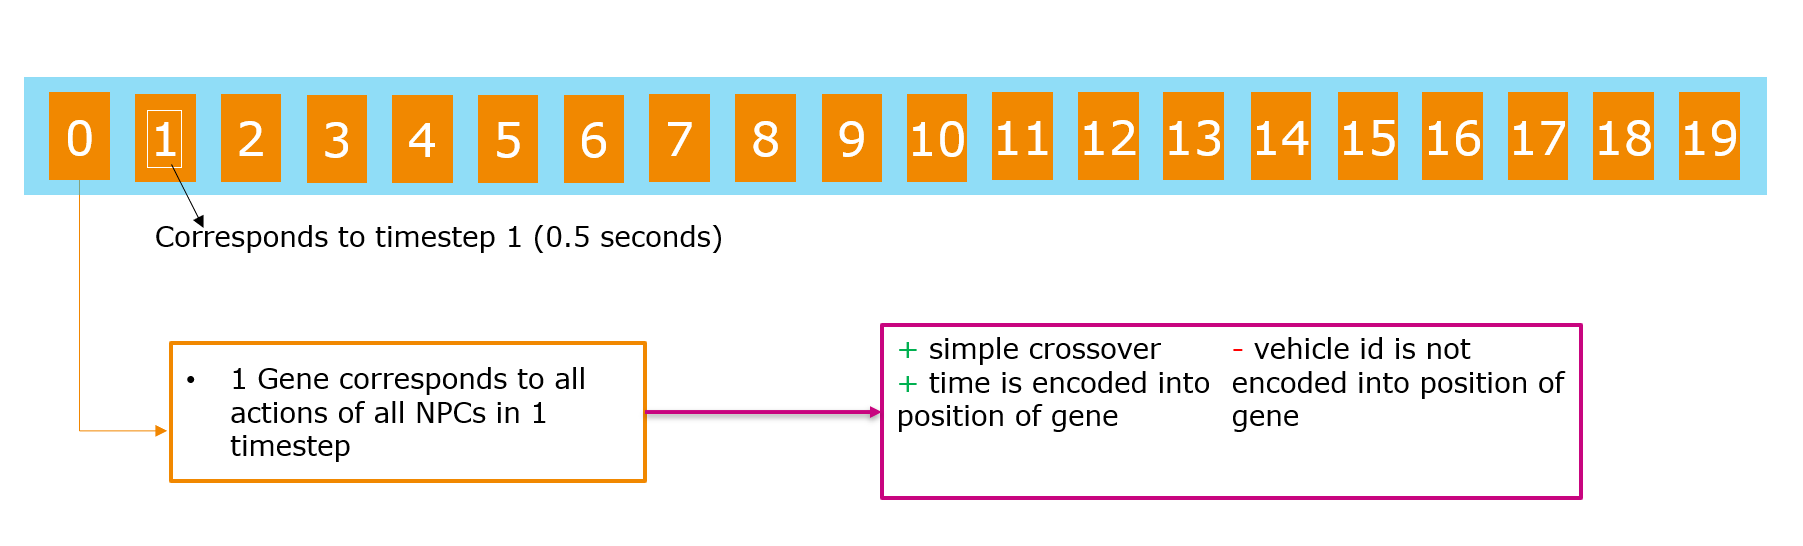
\includegraphics[width=1\linewidth]{figures/time_encoding}
	\caption{Time}
	\label{figure:encoding:chromosome:time}
\end{figure}


Given the previously stated simulation time of 35 seconds, each chromosome has a length of $35 * 2 = 70$ genes. Each gene consits of $number\_of\_actors$ actions.
Crossover can thus only move all actions of a timestep at once, modifing between actions of the same timestep can only be done using mutation. If this is desired will be seen in the next chapters.


\paragraph{TimeNPC}
The second encoding has the name "TimeNPC", and is somewhat differently structured. Now, genes only hold 1 action, encoding now not only the timestep, but also the actor id in the position of the gene inside the chromosome. Now, each actors actions will be listed one after another. This is visualized in figure \ref{figure:encoding:chromosome:time_npc}.

\begin{figure}[ht] 
	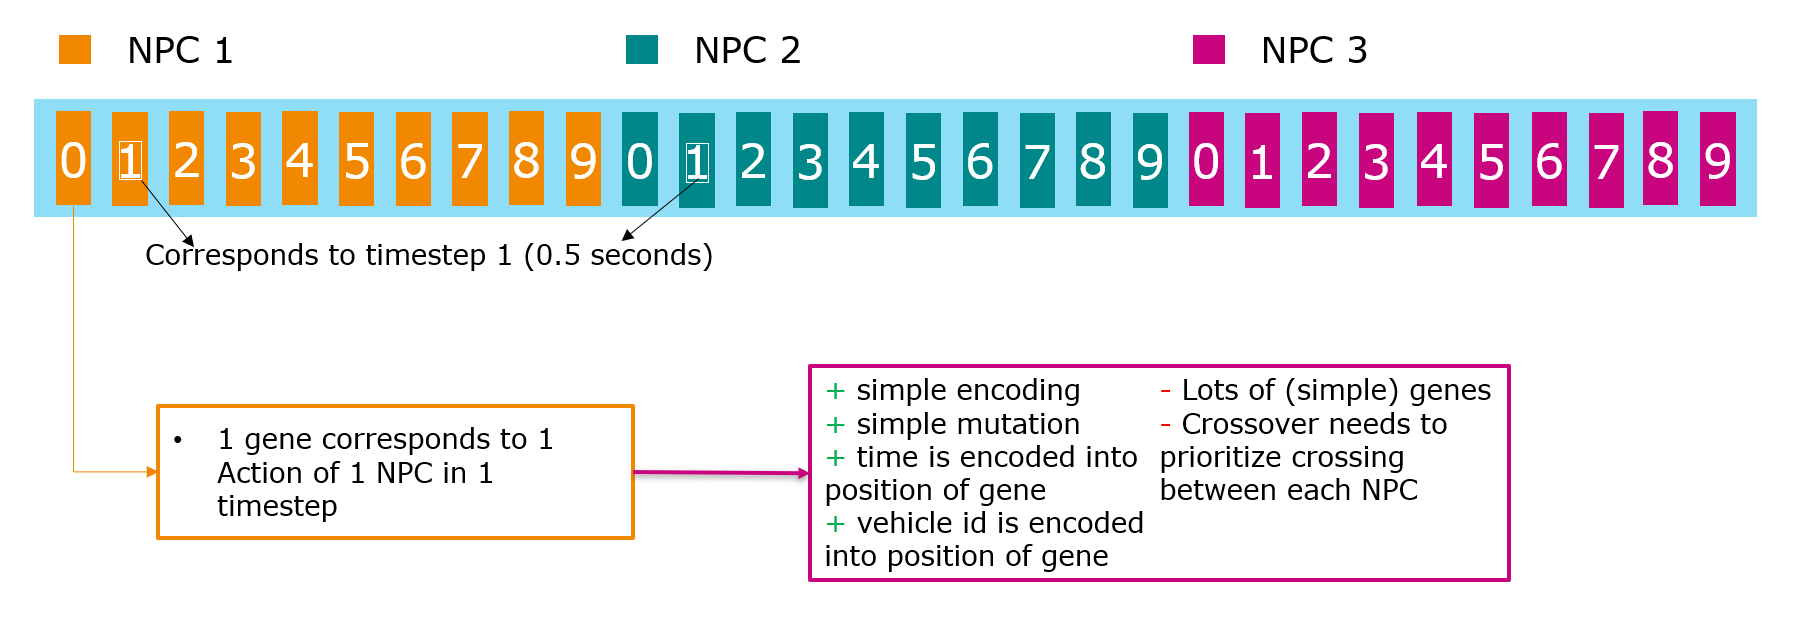
\includegraphics[width=1\linewidth]{figures/time_npc_encoding}
	\caption{Time + NPC}
	\label{figure:encoding:chromosome:time_npc}
\end{figure}

Now, each gene has a length of $1$ and each chromosome now has a length of $35 * 2 * number\_of\_actors$, which makes them much longer compared to the previous encoding. This now allows the crossover operation to modify only specific actions of one timesstep. Previously this was not possible.

However for this encoding to make sense, the crossover operations "OnePoint" and "TwoPoint" had to be modified as follows. In an example of 10 NPCs, the operations will be executed for each NPC separately. Otherwise these two operations would have only had an effect on 1 or 2 different NPCs. For the reaiming NPCs, their actions would stay the same.

\subsubsection{Gene}
Two different encodings for genes were implemented as well. A gene always consits of a list, which depending on the chromosome type either has a length of $number\_of\_actors$ (In case ChromosomeEncoding == Time) or of length 1 (in case ChromosomeEncoding == TimeNPC). The following two encodings thus show the type of object, which is in these lists.

\paragraph{Integer}
The first encoding uses integer, which are translated into actions when the simulation is started. For each action, a range of integers is assigned, the larger the range, the more likely the action is chosen by the GA. Actions that have parameters are split into different ranges, according to which paramters make sense. For example ModifyTargetVelocity is split into five different parts, with different percentages, namely 50, 70, 100, 130, 160. The range of integers assigned to these parts is different. A percentage setting of 100 for example has the largest integer range assigned.
In Appendix , the probabilty of an actions can be seen. In Appendix ... the probabitly per actions of the parameters can be viewed.

These ranges were assigned based on intuition and trial and error. The encoding is visualized in \ref{figure:encoding:gene:int}.

TODO: Due to the cliff problem, it was decided to not use binary representations for these integers. Due to the mutation choosing the integers randomly, it is not a problem that the variables are not really "continous".

\begin{figure}[ht] 
	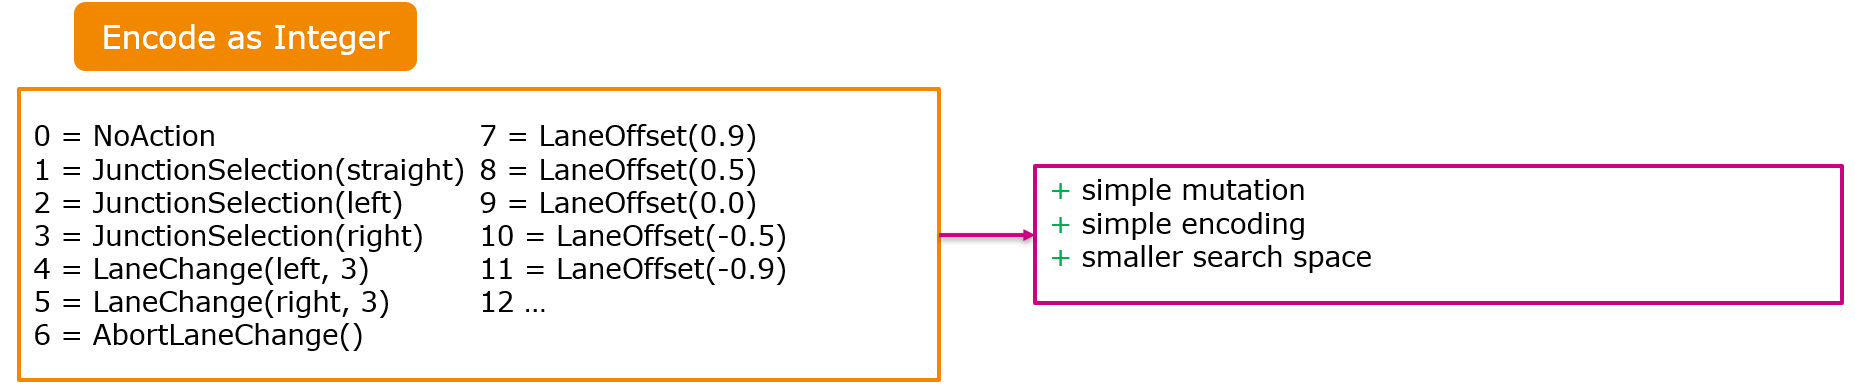
\includegraphics[width=1\linewidth]{figures/int_encoding}
	\caption{Integer}
	\label{figure:encoding:gene:int}
\end{figure}

\paragraph{Dictionary}
The second encoding is much similar to the actual actions used in the simulations. Now, no translation is necessary anymore. During generation of the individuals, each action is again selected based on different probabilities assigned to actions, which again can be viewed in Appendix ... . These probablilites are the same as for the integer encoding. However the difference is, in case an action has parameters that need to be chosen. 
For each parameter, a range and a randomness function was chosen. For example in case of the percenetage parameter in ModifyTargetVelocity, the values are selected from a GausDistribution, with mu= 100, sigma=25 and a range limit between 0 and 300.

Again, these probability functions with settings were assigned based on intuition as well as trial and error. Detailed information can be seen in Appendix...

Figure \ref{figure:encoding:gene:dict} shows a visualization.

\begin{figure}[ht] 
	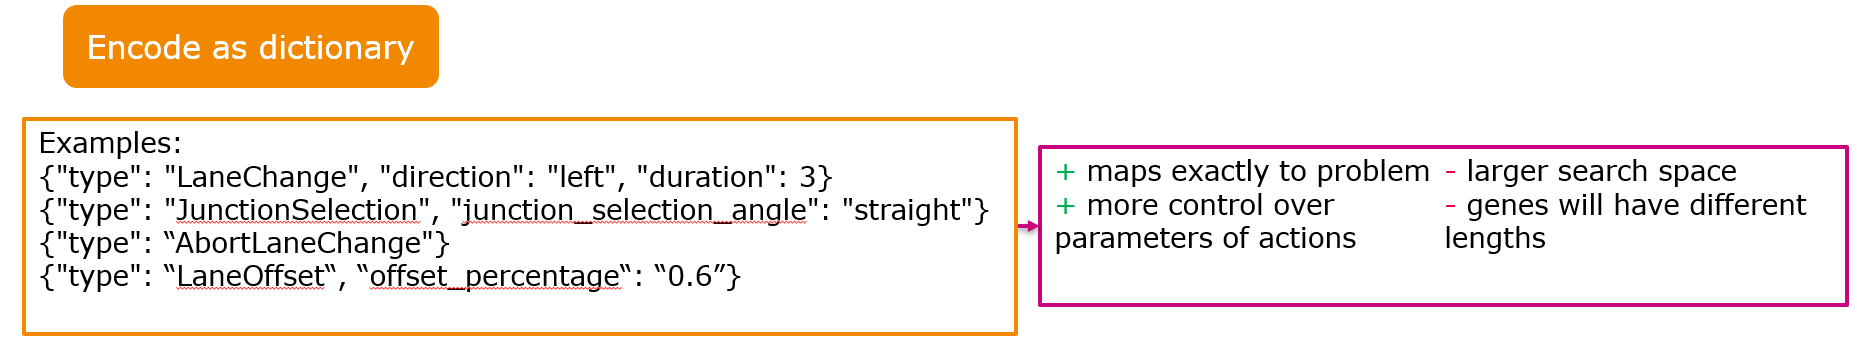
\includegraphics[width=1\linewidth]{figures/dict_encoding}
	\caption{Dictionary}
	\label{figure:encoding:gene:dict}
\end{figure}

\subsection{Cost Function}
\label{implementation:cost_function}
\todo{Suggestion florian: better explain cost values (e.g. 3500 means no emergency break...)}

Cost function is a bit difficult, as we are only using internal values. No ADAS/AD system is tested and we thus have to work with what we got.
This is the code of the cost function:

\begin{lstlisting}[language=Python, tabsize=4]
SEPS_PER_SECOND = 100
# allow emergency breaks to last only 3 seconds
MAX_DURATION = 3 * STEPS_PER_SECOND

cost = 0
duration_counter = 0
for i in range(len(result["ego_emergency_stop"])):
	if not result["ego_emergency_stop"][i]:
		# base cost in case of no current emergency break
		cost = cost + 1
		duration_counter = 0
	else:
		if duration_counter > MAX_DURATION:
			# increase cost if emergency break max duration is exceeded
			cost = cost + 10
		duration_counter += 1
return cost
\end{lstlisting}
result["ego\_emergency\_stop"] is a list with the length $100 * simulation\_duration\_seconds$ (because 100hz). It contains a boolean per step, if the EGO vehicle has initiated an emergency stop.

It would have been interesting to not only test for emergency stops (which will make the NPCs try to get the EGO to hard break often) but also improve time to collison (TTC), as was done by \todo{Ref florian}. However by the time of starting the testing, no working TTC functionality was implemented. Thus, only the emergency break cost function is used by the GA to be optimized.


TODO: rewrite
As previously defined, 1 simulations has a duration of 35 seconds. In order to simplify the evaluation of the cost values in Chapters \ref{chap:hyperparameter_tuning} and \ref{chap:evaluation}, the cost value will be inserted into the following equation

(3500 - cost) / 100

In the last chapter \ref{chap:hyperparameter_tuning}, values from the cost function (shown in section \ref{implementation:cost_function}) were displayed. These values however are difficult to interpret. Considering this, in this chapter, these values will be modified using this equation:

This will result in a value called Emergency Brake Duration, which will from now on be using instead of cost. The higher the Emergency Brake Duration, the better. It is important to consider, that this value might not exactly correspond to the actual Emergency Brake Duration time from the simulation, as the cost function applies a penalty for emergency breaks lasting longer then 3 seconds (again, see section \ref{implementation:cost_function}).

\section{Behavior Tree}
A behavior tree is a decision tree. \todo{insert a good introduction to BT}
Depending on the functionality under test, it is possible to let the EGO vehicle be controlled by a Behaviour Tree. This makes sense if for example a functionilty like AEB is tested, where only the breaks are controlled. In case of a full driving stack, no Behaviour Tree would be used.

The general idea is to have an EGO vehicle moving in a "relateable" manner trough the world. It will try to dodge standing or slow moving obstacles. This needs to be done in a determinisitc manner in order to no introduce randomness into the simulation.

For this, Behaviour Tree is used. While it has access to the same Action Interface (described in section \ref{implementation:action_interface}) as the Genetic Algorithm, it is more tightly integrated with the Traffic Manger. While the Genetic Algorithm only ingests the results generated by the Simulation with the cost function, the Behaviour Tree needs access to internal functions during the simulation. The following figure shows the behaviour tree implemented.




\iffalse
\begin{figure}[H]
	\centering
	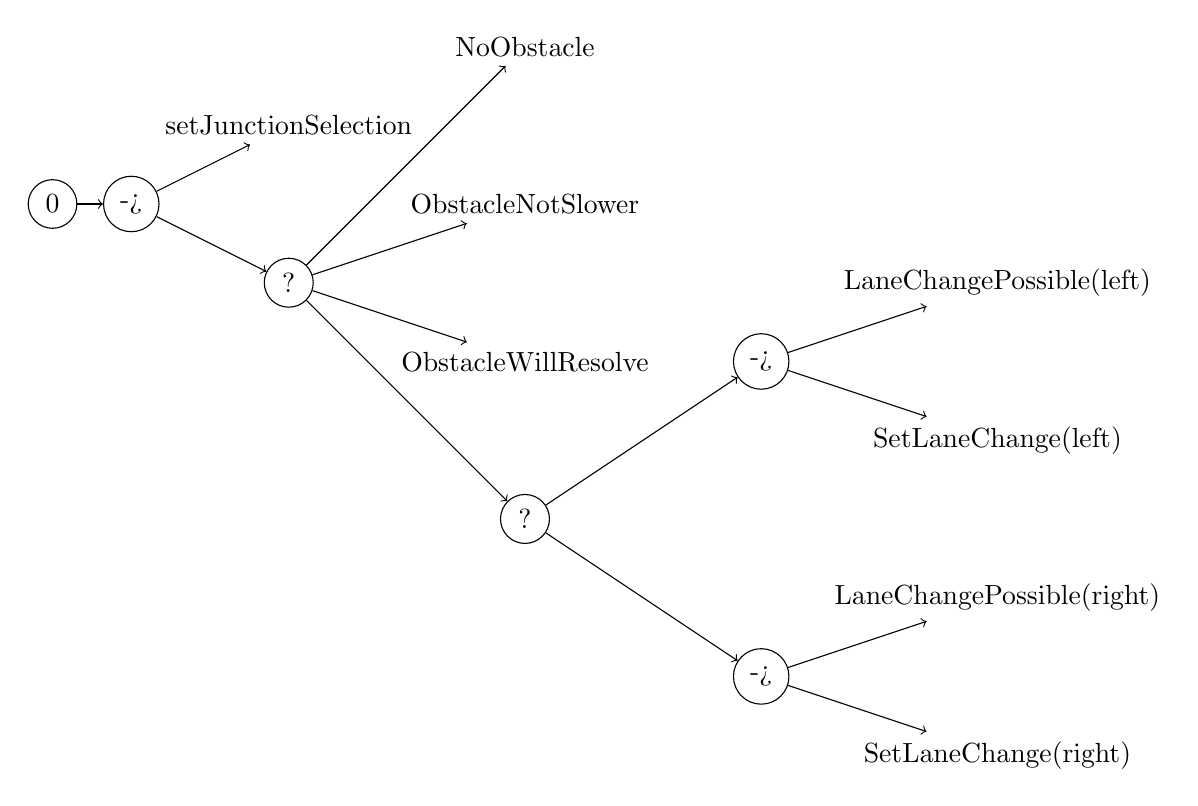
\begin{tikzpicture}
		% Define 1 2 3
		\node[draw, circle] (NodeStart) at (0,0) {0};
		\node[draw, circle] (Sequence1) at (1,0) {->};
		\draw[->] (NodeStart) -- (Sequence1);
		
		\node (Action1) at (3,1) {setJunctionSelection};
		\node[draw, circle] (OR1) at (3,-1) {?};
		\draw[->] (Sequence1) -- (Action1);
		\draw[->] (Sequence1) -- (OR1);

		\node (Action21) at (6,2) {NoObstacle};
		\node (Action22) at (6,0) {ObstacleNotSlower};
		\node (Action23) at (6,-2) {ObstacleWillResolve};
		\node[draw, circle] (OR2) at (6,-4) {?};
		\draw[->] (OR1) -- (Action21);
		\draw[->] (OR1) -- (Action22);
		\draw[->] (OR1) -- (Action23);
		\draw[->] (OR1) -- (OR2);
		
		\node[draw, circle] (Sequence31) at (9,-2) {->};
		\node[draw, circle] (Sequence32) at (9,-6) {->};
		\draw[->] (OR2) -- (Sequence31);
		\draw[->] (OR2) -- (Sequence32);
		
		\node (Action41) at (12,-1) {LaneChangePossible(left)};
		\node (Action42) at (12,-3) {SetLaneChange(left)};
		\node (Action43) at (12,-5) {LaneChangePossible(right)};
		\node (Action44) at (12,-7) {SetLaneChange(right)};
		\draw[->] (Sequence31) -- (Action41);
		\draw[->] (Sequence31) -- (Action42);
		\draw[->] (Sequence32) -- (Action43);
		\draw[->] (Sequence32) -- (Action44);
		
		
	\end{tikzpicture}
	\caption{Used Behaviour Tree}
\end{figure}
\fi

\begin{figure}[ht]
	\centering
	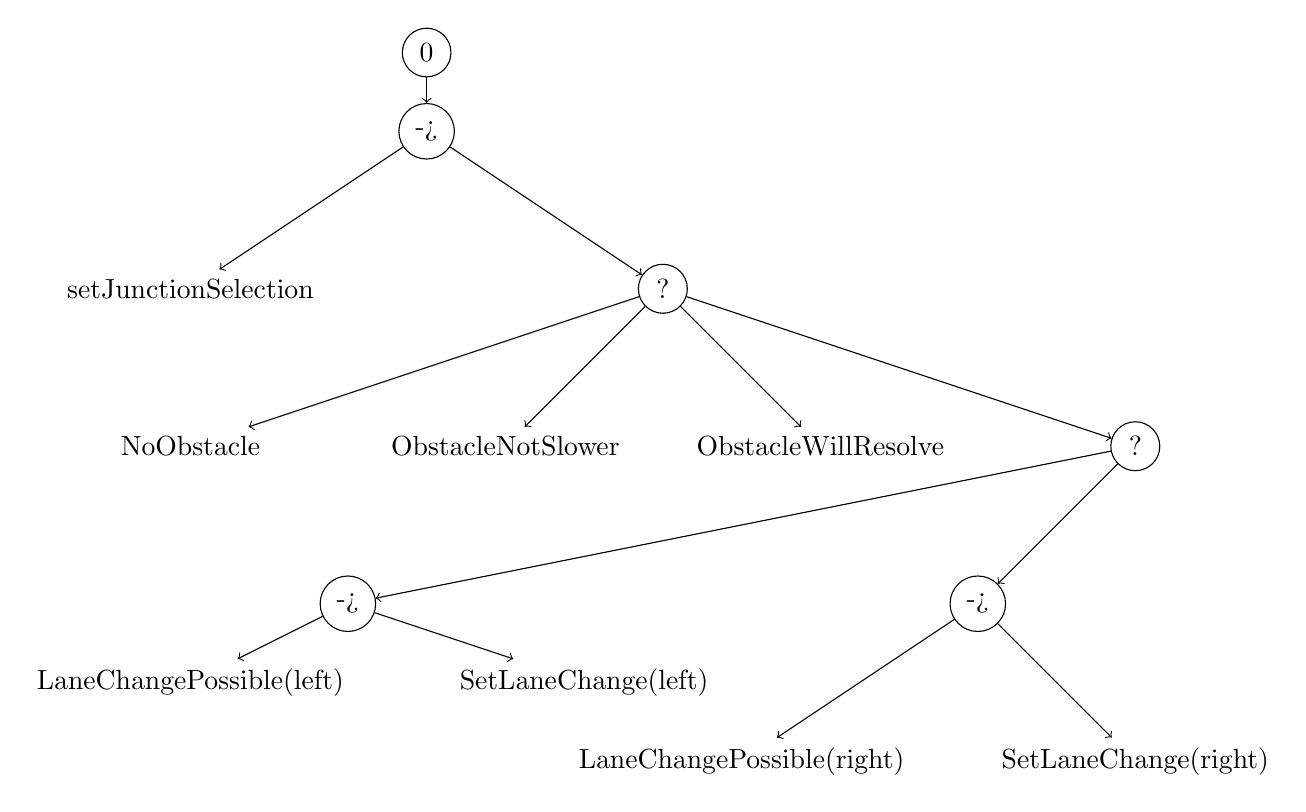
\begin{tikzpicture}
		% Define 1 2 3
		\node[draw, circle] (NodeStart) at (0,0) {0};
		\node[draw, circle] (Sequence1) at (0,-1) {->};
		\draw[->] (NodeStart) -- (Sequence1);
		
		\node (Action1) at (-3,-3) {setJunctionSelection};
		\node[draw, circle] (OR1) at (3,-3) {?};
		\draw[->] (Sequence1) -- (Action1);
		\draw[->] (Sequence1) -- (OR1);
		
		\node (Action21) at (-3,-5) {NoObstacle};
		\node (Action22) at (1,-5) {ObstacleNotSlower};
		\node (Action23) at (5,-5) {ObstacleWillResolve};
		\node[draw, circle] (OR2) at (9,-5) {?};
		\draw[->] (OR1) -- (Action21);
		\draw[->] (OR1) -- (Action22);
		\draw[->] (OR1) -- (Action23);
		\draw[->] (OR1) -- (OR2);
		
		\node[draw, circle] (Sequence31) at (-1,-7) {->};
		\node[draw, circle] (Sequence32) at (7,-7) {->};
		\draw[->] (OR2) -- (Sequence31);
		\draw[->] (OR2) -- (Sequence32);
		
		\node (Action41) at (-3,-8) {LaneChangePossible(left)};
		\node (Action42) at (2,-8) {SetLaneChange(left)};
		\node (Action43) at (4,-9) {LaneChangePossible(right)};
		\node (Action44) at (9,-9) {SetLaneChange(right)};
		\draw[->] (Sequence31) -- (Action41);
		\draw[->] (Sequence31) -- (Action42);
		\draw[->] (Sequence32) -- (Action43);
		\draw[->] (Sequence32) -- (Action44);
		
		
	\end{tikzpicture}
	\caption{Used Behaviour Tree}
\end{figure}


Starting out, \todo{Explain BT}

